\documentclass[11pt]{article}
\usepackage[margin=1in]{geometry}
\usepackage{volfit_preamble}
\graphicspath{{figures/}}

\title{\textbf{Wings, Lee Bounds and Tail Control}\\[2pt]
\large How four models keep their extrapolated wings arbitrage-admissible\\[2pt]
\normalsize Vol-Fitter Technical Notes, No.~09}
\author{Vol-Fitter}
\date{\today}

\begin{document}
\maketitle
% Auto-generated by gen_wings.py — do not edit.
\newcommand{\betaLQDL}{0.0971}
\newcommand{\betaLQDR}{0.0358}
\newcommand{\betaSVIL}{0.1093}
\newcommand{\betaSVIR}{0.0364}
\newcommand{\betaMCSIVL}{0.1057}
\newcommand{\betaMCSIVR}{0.0297}
\newcommand{\sviwingLraw}{0.1093}
\newcommand{\sviwingRraw}{0.0364}


\begin{abstract}
A smile model earns its keep in the \emph{wings} --- the region beyond the
quoted strikes, where the fit becomes pure extrapolation and where mispriced
tails leak into var-swaps, risk-reversals and butterflies. This cross-cutting
note collects the wing treatment shared by the Vol-Fitter's models. The
universal constraint is Lee's moment formula: the asymptotic slope of total
implied variance, $\beta=\limsup_{k\to\pm\infty}w(k)/|k|$, cannot exceed $2$
and is tied to the moment critical exponents by the explicit map
$\beta=\psi(p)$. We show how each model realizes or enforces it --- LQD
structurally, SVI by a soft cap, the Multi-Core Sigmoid (MCS) by wing-neutral
hats --- and prove the zero-wing inheritance the MCS design relies on. The finite wing is a
separate battle: the asymptotic slope can be admissible while a hat still
dents the Durrleman density out where quotes are sparse, which is why the
default-on put-wing regularizer samples $g$ \emph{past} the traded range
(measured: worst violation $-10.2\to-0.008$ on the synthetic slice, a
$\sim400\times$ median repair on real illiquid wings, byte-identical on clean
slices). A case file replays the backtest finding that motivated it and the
ablation verdict that the de-Americanization repair and the penalty are
complementary, not redundant ($92\to25$ bp with the input repair alone;
$749$ bp with the output penalty alone; $225$ bp with both). The note closes
with the arc's centerpiece: the \emph{confinement principle} --- which
no-arbitrage constraints must be sampled only where data lives, and which
must extend into the wings --- with its four production instances.
\end{abstract}

\tableofcontents
\newpage

%======================================================================
\section{The production problem}
\label{sec:problem}

Nobody quotes the far wings, yet everything downstream reads them: var-swap
replication integrates $1/K^2$-weighted prices into the tails, risk metrics
difference the wings, and the graph extrapolator (Note~14) inherits whatever
tail the fitted model draws. Wing errors are invisible in the fit RMS ---
there are no quotes to miss --- and show up later as a mispriced tail
somewhere else. Two distinct things can go wrong: the \emph{asymptotic} slope
can violate Lee's model-free bound (an arbitrage against the existence of any
law), and the \emph{finite} wing can lose density positivity even with an
admissible slope (a butterfly arbitrage in the extrapolated region).

\begin{invariant}
\begin{enumerate}[leftmargin=1.6em]
\item Every displayed wing is Lee-admissible: $\beta\le2$, structurally where
possible, by a soft cap otherwise.
\item Single-slice (butterfly) constraints \emph{extend} into the wings;
two-slice (calendar) constraints are \emph{confined} to the traded range
(\cref{sec:principle}).
\item Every wing guard is strictly additive: on an already-clean slice it is
byte-identical to no guard.
\item The tail is a property of the model's extrapolation law, not of the
quotes; where the desk needs control (LV deep puts), the slope is an explicit
knob or a calibrated variable.
\end{enumerate}
\end{invariant}

%======================================================================
\section{The universal constraint: Lee's moment formula}
\label{sec:lee}

Let $w(k,T)=\sigma_{\BS}^2(k,T)\,T$ be total implied variance at log-moneyness
$k=\log(K/F_T)$.

\begin{theorem}[Lee moment formula \cite{Lee2004}]
\label{thm:lee}
Define the wing slopes
\[
\beta_R=\limsup_{k\to+\infty}\frac{w(k,T)}{k},\qquad
\beta_L=\limsup_{k\to-\infty}\frac{w(k,T)}{|k|},
\]
and let $p_R^*=\sup\{p:\E[S_T^{1+p}]<\infty\}$ and
$q_L^*=\sup\{q:\E[S_T^{-q}]<\infty\}$ be the moment critical exponents. Then
\begin{equation}
\beta_R=\psi(p_R^*),\qquad \beta_L=\psi(q_L^*),\qquad
\psi(p)=2-4\big(\sqrt{p^2+p}-p\big).
\label{eq:psi}
\end{equation}
\end{theorem}

\begin{lemma}[Properties of the Lee map]
\label{lem:psi}
$\psi$ is a strictly decreasing bijection from $[0,\infty]$ onto $[0,2]$,
with $\psi(0)=2$, $\psi(\infty)=0$, and explicit inverse
$p=\tfrac{1}{2\beta}+\tfrac{\beta}{8}-\tfrac12$. In particular $0\le\beta\le2$
for \emph{every} arbitrage-free smile --- the ceiling $\beta=2$ is model-free.
\end{lemma}

\begin{proof}
Write $\psi(p)=2\big(\sqrt{p+1}-\sqrt p\big)^2$: the parenthesis is positive
and strictly decreasing (its derivative
$\tfrac12(1/\sqrt{p+1}-1/\sqrt p)<0$), with limits $1$ at $p=0$ and $0$ at
$\infty$; squaring and doubling gives the range $(0,2]$ plus the endpoint
$\psi(\infty)=0$. Solving $\beta=2(\sqrt{p+1}-\sqrt p)^2$ for $p$ gives the
stated inverse by elementary algebra.
\end{proof}

The map, and the way LQD reads its slopes off the endpoint scales
$A_L=e^{g(0)}$, $A_R=e^{g(1)}$ of Note~01, are a few lines. \Cref{app:ref}
verifies this distilled listing against the production \texttt{lee\_psi}
and \texttt{lee\_slopes} to $10^{-15}$ (the production function takes the
LQD parameter object and computes the endpoint scales itself):

\begin{lstlisting}[caption={Lee's $\psi$ and the LQD structural wing slopes
(distilled from \texttt{models/lqd/basis.py}).},label={lst:lee}]
def lee_psi(p):                 # beta = psi(p); decreasing, psi(0)=2
    return 2 - 4*(np.sqrt(p*p + p) - p)

def lee_slopes(A_L, A_R):       # exponential tails -> exact exponents
    beta_L = lee_psi(1/A_L)                          # left:  p* = 1/A_L
    beta_R = 2.0 if A_R >= 1 else lee_psi(1/A_R - 1) # right: p* = 1/A_R - 1
    return beta_L, beta_R
\end{lstlisting}

\begin{figure}[H]
\centering
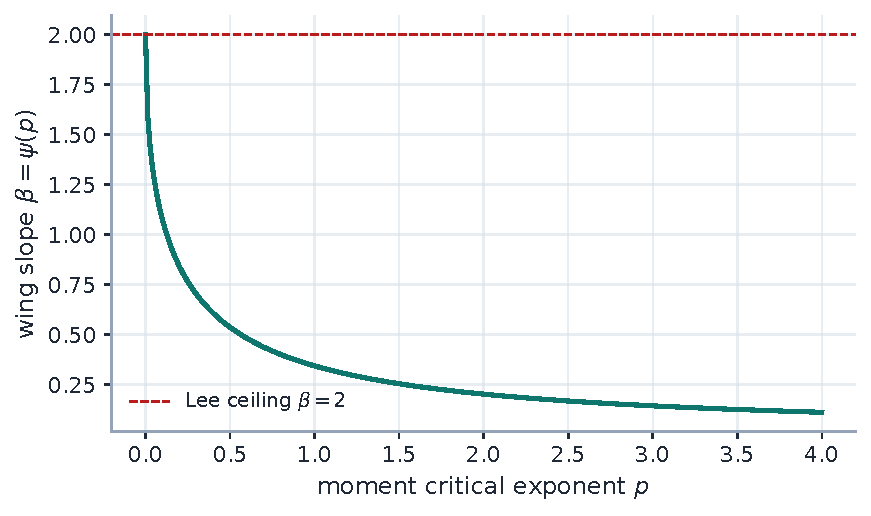
\includegraphics[width=0.62\textwidth]{fig_wings_psi.pdf}
\caption{The Lee map $\beta=\psi(p)$: heavier tails (smaller moment exponent
$p$) force steeper variance wings, capped at the model-free ceiling
$\beta=2$.}
\label{fig:psi}
\end{figure}

\begin{heuristic}
The wing slope and the tail heaviness are two faces of one coin. A fat right
tail (few finite positive moments) \emph{must} show up as a steep right
variance wing; a model that draws a flat wing over a fat-tailed density is
internally inconsistent and will misprice far-OTM calls. Lee's bound is not a
nuisance constraint but a consistency condition between the smile and the law
it implies --- which is why the LQD model, built from the law outward,
satisfies it automatically.
\end{heuristic}

%======================================================================
\section{Four models, four wing mechanisms}
\label{sec:models}

\subsection{LQD: Lee-consistent by construction}

The LQD model (Note~01) parametrizes the log quantile density with
logarithmic endpoints, giving \emph{exponential} return tails with scales
$A_L,A_R$ read off the endpoint coefficients. The moment exponents are exact,
$p_R^*=1/A_R-1$ and $q_L^*=1/A_L$, and the wing slopes follow from
\cref{thm:lee}:
\begin{equation}
\beta_L=\psi(1/A_L),\qquad \beta_R=\psi(1/A_R-1),\quad A_R<1.
\label{eq:lqd_wings}
\end{equation}
No penalty enforces this --- it is structural. The only wing-related
constraint is the hard $A_R<1$ (finite forward), handled by Note~01's soft
barrier. The benchmark fit yields $(\beta_L,\beta_R)=(\betaLQDL,\betaLQDR)$.

\subsection{SVI: linear wings with a soft cap}

Raw SVI (Note~02) has exactly linear wings, $w(k)\sim b(1\mp\rho)|k|$, so
$\beta_L=b(1-\rho)$ and $\beta_R=b(1+\rho)$ in closed form
($=(\sviwingLraw,\sviwingRraw)$ on the benchmark parameters). Lee's bound is
the explicit inequality $b(1+|\rho|)\le2$, enforced as a soft hinge
$\max\big(b(1+|\rho|)-\beta_{\max},0\big)$ at weight $10^3$ alongside the
min-variance penalty (cap \texttt{leeSlopeMax}$\,=2$). On any admissible
smile both penalties are exactly zero; they only fence the optimizer out of
the inadmissible region.

\subsection{Multi-Core Sigmoid (MCS): inherited wings}

The Multi-Core Sigmoid (MCS) slice (Note~03) is a convex base plus up to two
\emph{zero-wing} hats.

\begin{proposition}[Zero-wing inheritance]
\label{prop:zerowing}
Let $v(z)=v_{\text{base}}(z)+\sum_r h_r(z)$ in standardized moneyness $z$,
where each hat $h_r$ and its first two derivatives vanish as
$z\to\pm\infty$. Then the asymptotic variance slopes of $v$ equal those of
the base, $S_0\mp2K_0/\kappa_{P,C}$, for \emph{any} number of hats and any
hat parameters; in total-variance $k$-space, with
$k=\sigma_{\text{ref}}\sqrt t\,z$ and $w=tv$,
\begin{equation}
\beta_{L,R}
=\frac{\sqrt t}{\sigma_{\text{ref}}}\,
\Big|S_0\mp\frac{2K_0}{\kappa_{P,C}}\Big|.
\label{eq:siv_wings}
\end{equation}
\end{proposition}

\begin{proof}
$v'(z)=v'_{\text{base}}(z)+\sum_rh_r'(z)\to v'_{\text{base}}(z)$ as
$|z|\to\infty$ since each $h_r'\to0$; the base is asymptotically linear with
the stated slopes. The $k$-space conversion is the chain rule through
$k=\sigma_{\text{ref}}\sqrt t\,z$ and $w=tv$.
\end{proof}

On the benchmark, $(\beta_L,\beta_R)=(\betaMCSIVL,\betaMCSIVR)$. Adding cores
cannot change the wings --- the entire point of the zero-wing design. But the
proposition pins only the asymptotic \emph{slope}: a hat can still dent the
Durrleman $g$ below zero at \emph{finite} $|z|$, out in the sparsely quoted
put wing. That residual failure mode is real, measured, and policed by the
put-wing regularizer of \cref{sec:r6}.

\subsection{Local volatility: controlled linear extrapolation}

The piecewise-affine local-vol surface (Note~04) has no closed-form
implied-vol wing. Beyond the deepest strike vertex it extrapolates the
\emph{local} variance linearly with slope \texttt{left\_extrap\_a} times the
first interior cell's slope; the right wing is flat-clamped. The knob mapping
is deliberate: the slope is $0$ (flat clamp) on the hot path, seeded from
\texttt{leftWingSlopeMult}$\,=1.5$ when the convex-wing hinge is on, and
becomes a \emph{free calibration variable} (bounds $[0,20]$) exactly when a
var-swap quote is present to identify the deep-put tail --- the one
instrument that genuinely observes it (Note~08).

\subsection{Side by side}

\Cref{fig:extrap} fits the same narrow window with the three parametric
models and extrapolates far past it. The wings agree in sign (the equity put
skew, $\beta_L>\beta_R$) and order of magnitude but diverge in detail ---
each tail is a property of \emph{its} extrapolation law, not of the identical
quotes. That divergence is not a defect to be averaged away: past the last
quote a wing is a modelling \emph{choice}, not an estimate --- the far wing is
exactly where a model extrapolates with confidence it does not have --- so
what the fitter guarantees is not agreement but a stated, tested \emph{wing
contract} per model. LQD draws exponential return tails with structural
slopes $\psi(1/A_L),\psi(1/A_R-1)$; SVI draws linear variance wings
$b(1\mp\rho)$ under the soft Lee cap; the MCS base alone owns the tails, hats
neutral (\cref{prop:zerowing}); LV extrapolates local variance flat on the
call side and controlled-linearly on the put side. Choosing a model \emph{is}
choosing an extrapolation law --- the differences are the point; the shared
promise is only that every contract is Lee-admissible.
\Cref{tab:betas} collects the analytic slopes.

\begin{figure}[H]
\centering
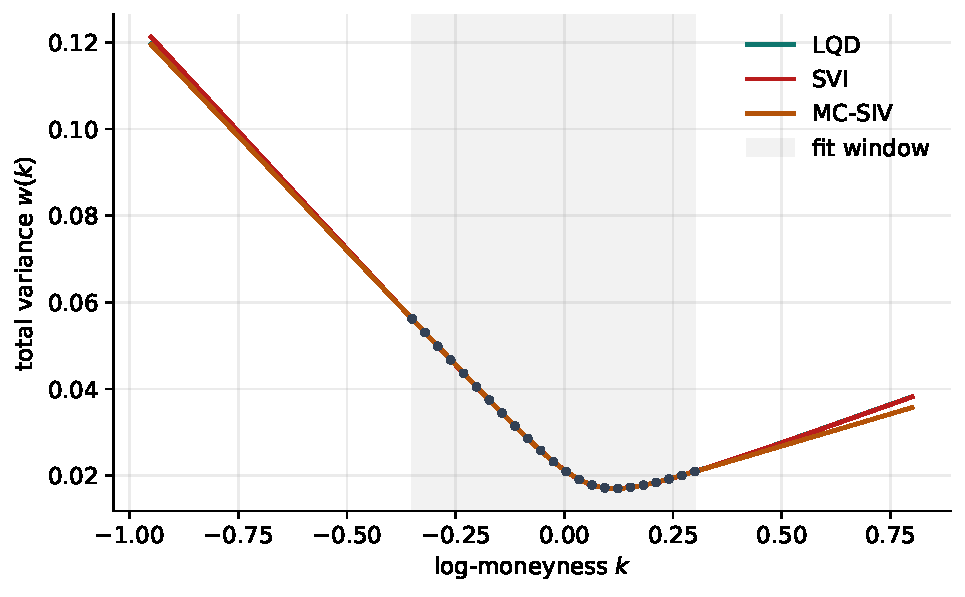
\includegraphics[width=0.85\textwidth]{fig_wings_extrap.pdf}
\caption{Three models fitted to the same window (shaded) and extrapolated.
Inside the window they agree to vol bps; outside, each draws its own
Lee-admissible wing. The divergence \emph{is} the model choice.}
\label{fig:extrap}
\end{figure}

\begin{table}[H]
\centering
\caption{Analytic asymptotic total-variance wing slopes
$\beta=\lim w(k)/|k|$ on the benchmark window; all far below the Lee ceiling
$2$.}
\label{tab:betas}
\begin{tabular}{lrrr}
\toprule
Model & $\beta_L$ (put) & $\beta_R$ (call) & mechanism\\
\midrule
LQD & \betaLQDL & \betaLQDR & structural via $\psi(1/A)$\\
SVI & \betaSVIL & \betaSVIR & linear $b(1\mp\rho)$, soft Lee cap\\
MCS & \betaMCSIVL & \betaMCSIVR & base wings, hats neutral
(\cref{prop:zerowing})\\
\bottomrule
\end{tabular}
\end{table}

%======================================================================
\section{Policing the finite wing: the MCS put-wing regularizer}
\label{sec:r6}

An admissible slope does not make an admissible wing. The backtest's arb
census located the MCS's failures precisely: $64\%$ of butterfly
violations sit in the \emph{put} wing (median worst-violation location
$z\approx-3.2$), against $4\%$ at the money --- hats fitted to sparse
illiquid quotes buy in-sample RMS by denting the density where no quote
objects. The shipped defence (the R6 fix) has three parts:

\begin{enumerate}[leftmargin=1.6em]
\item \textbf{A capacity cap.} \texttt{nCores} is clamped to $\le2$ at the
schema (and to $(n_{\text{quotes}}-6)/4$ in the calibrator): most historical
violations came from high-core fits chasing noise.
\item \textbf{A one-sided Durrleman hinge.} The refine stage carries residual
rows $\sqrt{\lambda_{\text{w}}}\,\max(-g(z_m),0)$ on a $49$-point grid
extending \emph{two standardized-moneyness units past the traded range} on
both sides, with the put side weighted $2\times$ (where the census says the
risk lives). The weight is
$\lambda_{\text{w}}=(\texttt{sivWingPenaltyPct}/100)\cdot10^3$, default
$100\%$.
\item \textbf{A hybrid Jacobian.} The $g$ rows are finite-differenced (49
points, one column at a time) while the quote/ridge/calendar blocks keep
their analytic Jacobian --- the penalty costs little and perturbs nothing
when inactive.
\end{enumerate}

Measured: the synthetic arb slice's worst $g$ went $-10.2\to-0.008$; on real
illiquid wings (EEM) the median worst violation improved $\sim400\times$
($-7.86\to-0.019$) at $+79$ bp in-sample cost; on clean liquid slices the
penalty rows are zero and the fit is byte-identical to $3\times10^{-17}$.
Note that sampling $g$ \emph{past} the quoted range here is correct, not a
violation of confinement --- see \cref{sec:principle}.

\begin{example}[title={Case file: the MCS that invented a put wing}]
\textbf{Setup.} The three-regime backtest sweep (F4): the Multi-Core Sigmoid
on illiquid single names, where the put wing has a handful of wide quotes.

\textbf{Failure mode.} MCS-2 improved in-sample RMS over MCS-0 --- and
carried genuine butterfly arbitrage on $76\%$ of arb-prone nodes, almost all
in the put wing. The model was buying RMS with a fake weekend wing: a hat
parked where no quote could object.

\textbf{Diagnosis.} The analytic (FD-free) arb metric (R2) separated real
violations from finite-difference noise: with exact $w',w''$ per model, the
apparent LQD ``violations'' vanished entirely ($28\%\to0$ --- structural
positivity confirmed) while MCS-2's survived ($76\%$, genuine). The census
then localized them: put wing, $z\approx-3.2$.

\textbf{Fix.} The 2-core cap plus the put-weighted Durrleman hinge above
(output side), composing with the de-Americanization wing repair of Note~05
(input side).

\textbf{Verdict (ablation, test-locked).} On the arb-prone illiquid
population, with neither fix: worst $g$ $-30.4$, arbitrage on $100\%$,
in-sample $92$ bp. Input repair alone: arbitrage cut $\sim3\times$ \emph{and}
RMS improved to $25$ bp --- the MCS had been chasing arbitraged de-Am
inputs. Output penalty alone: arbitrage essentially eliminated
($g\ge-0.02$) but at $749$ bp --- brutal, because the model must fight its
own corrupted inputs. Both: the penalty's arbitrage removal at $225$ bp.
(Those are medians across the $38$ arb-prone census nodes; one real node
makes it concrete --- EFA in the Aug-2024 vol spike, $11$ days out, $22$
quotes: $75$ bp at $g=-116$ with neither defence, $18$ bp but $g=-12$ with
the repair alone, arb-free at $726$ bp with the penalty alone, arb-free at
$34$ bp with both.) \emph{Complementary, not redundant}: the input repair
makes the output penalty affordable. On liquid names both are byte-identical
no-ops.
\end{example}

%======================================================================
\section{The confinement principle}
\label{sec:principle}

Four production incidents --- the phantom calendar violations (Note~10's
case file), the local-vol convex-wing regression (Note~04), the de-Am global
repair revert (Note~05), and the MCS put-wing penalty above --- resolve into
one rule.

\begin{heuristic}
\textbf{The confinement principle.} \emph{A constraint that compares two
curves must be sampled only where data pins both; a constraint intrinsic to
one curve must hold everywhere, wings included.} A two-curve constraint
evaluated where both sides are extrapolation can only compare two fictions
--- any ``violation'' there is an artefact of the extrapolation laws, and
enforcing it lets the fiction corrupt the fit where data \emph{does} live. A
single-curve constraint (density positivity, call convexity) is a property of
the law itself: it has no rival extrapolation to be spuriously violated
against, and abandoning it in the wings is exactly how fake tails are born.
\end{heuristic}

\begin{center}
\small
\begin{tabular}{p{0.30\textwidth}p{0.13\textwidth}p{0.22\textwidth}p{0.24\textwidth}}
\toprule
Constraint & Curves & Treatment & Where\\
\midrule
Calendar floor $w_{\text{far}}\ge w_{\text{near}}$ & two &
\textbf{confined} to traded range & Note~10
(\nolinkurl{variance_floor_grid_from})\\
LV convex-wing hinge & two\footnotemark & \textbf{confined} to the
extrapolation tail below the deepest quote & Note~04\\
MCS Durrleman $g\ge0$ & one & \textbf{extended} $\pm2$ ATM-std past quotes &
\cref{sec:r6}\\
De-Am call convexity & one & \textbf{extended} to the wings, but
band-constrained and ATM-core-fixed & Note~05\\
\bottomrule
\end{tabular}
\end{center}
\footnotetext{The LV wing hinge compares the model's wing against the
\emph{quotes'} implied shape when sampled inside the quoted range --- the
regression of Note~04 --- so it behaves as a two-curve constraint and is
confined; in the pure extrapolation tail it degenerates to a one-curve
convexity preference, which is where it is allowed to act.}

The de-Am row shows the principle's refinement rather than an exception: the
constraint (convexity) rightly extends into the wings, but the
\emph{correction} it licenses is confined --- to the quoted bid--ask band and
away from the ATM core --- because a repair, unlike a constraint, moves
prices. Extending a one-curve constraint is safe; extending a repair's
\emph{authority} unboundedly is how a $27\%$ put wing became $104\%$
(Note~05).

\begin{remark}[Open problem: softer two-curve enforcement in the wings]
\label{rem:softwings}
Confinement as stated is binary: a two-curve constraint is either sampled
(inside the traded range) or ignored (outside). But the extrapolated region
is not uniformly worthless --- just past the last quote the options still
carry genuine premium, and there a calendar inversion between two
\emph{stated} wing contracts (\cref{sec:models}) is a real inconsistency
even if no quote witnesses it. Whether two-curve constraints deserve a
\emph{softer} enforcement in the near-extrapolation region --- the penalty
weight decaying with distance past the last quote, or with remaining time
value, so gross contract disagreements are still leaned on while deep-wing
phantoms stay harmless --- is open (flagged 2026-07). It must be settled
jointly with this note's wing contracts and Note~10's floor-grid
construction; see the matching open problem there.
\end{remark}

%======================================================================
\section{What is original here}
\label{sec:original}

The Lee theory is classical; the contribution is the \emph{uniform}
treatment. The same slope $\beta$ is computed three structurally different
ways (\eqref{eq:lqd_wings}, the SVI closed forms, \eqref{eq:siv_wings}) and
shown to agree on one window, so the model choice is a choice of \emph{how}
to extrapolate, never \emph{whether} the extrapolation is admissible. The
put-wing regularizer is a census-guided constraint --- placed where the
measured violations live, weighted by their measured asymmetry, and validated
by an ablation that also proved it composes with the input-side repair. And
the confinement principle of \cref{sec:principle} --- with its two-curve /
one-curve criterion --- turns four hard-won production incidents into one
transferable design rule.

%======================================================================
\section{Traceability}
\label{sec:traceability}

\begingroup
\small
\setlength{\tabcolsep}{3pt}
\begin{longtable}{@{}p{0.30\textwidth}p{0.12\textwidth}p{0.26\textwidth}p{0.28\textwidth}@{}}
\caption{Claims in this note and the code/tests that lock them.}\\
\toprule Claim & Object & Code anchor & Test anchor\\ \midrule
\endfirsthead
\toprule Claim & Object & Code anchor & Test anchor\\ \midrule
\endhead
LQD structural Lee slopes; underflow-safe &
\eqref{eq:lqd_wings} &
\nolinkurl{models/lqd/basis.py} &
\nolinkurl{test_lqd_basis.py::test_svi_fit_lee_slopes_match_note}, \nolinkurl{::test_lee_slopes_handle_underflowed_endpoint_scales}\\
SVI Lee cap enforced &
\cref{sec:models} &
\nolinkurl{models/svi_jw/calibrate.py} &
\nolinkurl{test_svi_calibrate.py::test_respects_lee_wing_bound}\\
MCS hats are zero-wing &
\cref{prop:zerowing} &
\nolinkurl{models/sigmoid/sigmoid.py}, \nolinkurl{kernels.py} &
\nolinkurl{test_sigmoid_model.py}\\
2-core cap &
\cref{sec:r6} &
\nolinkurl{api/schemas.py}, \nolinkurl{models/sigmoid/calibrate.py} &
\nolinkurl{test_siv_wing_penalty.py::test_cores_clamped_to_two}\\
Put-wing hinge removes wing arb; byte-identical on clean slices &
\cref{sec:r6} &
\nolinkurl{models/sigmoid/calibrate.py} &
\nolinkurl{test_siv_wing_penalty.py::test_penalty_removes_wing_arb}, \nolinkurl{::test_penalty_byte_identical_on_arb_free_slice}\\
Analytic FD-free arb metric &
\cref{sec:r6} &
\nolinkurl{backend/backtest/dispatch.py}, \nolinkurl{models/sigmoid/kernels.py} &
\nolinkurl{test_backtest_arb.py}\\
R3$\times$R6 ablation: complementary &
case file &
\nolinkurl{backend/backtest/ablation_arb.py} &
\nolinkurl{test_ablation_arb.py}\\
De-Am wing repair (input side) &
\cref{sec:principle} &
\nolinkurl{calib/convex_deam.py} &
\nolinkurl{test_convex_deam.py}\\
Calendar floor confined (two-curve) &
\cref{sec:principle} &
\nolinkurl{calib/calendar.py} &
\nolinkurl{test_overlay_calendar.py::test_wide_grid_breaks_svi_but_data_grid_does_not}\\
LV convex wing confined to tail &
\cref{sec:principle} &
\nolinkurl{api/affine_fit.py} &
\nolinkurl{test_affine_grid_design.py::test_convex_wing_confined_to_quoted_extrapolation}\\
\bottomrule
\end{longtable}
\endgroup

\appendix
%======================================================================
\section{Hyperparameter atlas}
\label{app:atlas}

\begin{longtable}{p{0.27\textwidth}p{0.13\textwidth}p{0.51\textwidth}}
\caption{Wing-related knobs (cross-model).}\label{tab:atlas}\\
\toprule Knob & Default & Role\\ \midrule
\endfirsthead \toprule Knob & Default & Role\\ \midrule \endhead
\multicolumn{3}{l}{\emph{Surfaced}}\\ \midrule
\texttt{sivWingPenaltyPct} & $100$ & Put-wing Durrleman hinge strength
(\% of the $10^3$ base weight); $0$ disables.\\
\texttt{nCores} & $2$ (max $2$) & MCS core count, schema-clamped
(\cref{sec:r6}).\\
\texttt{leeSlopeMax} & $2.0$ & SVI Lee cap $b(1+|\rho|)\le\beta_{\max}$.\\
\texttt{sviPenaltyWeight} & $10^3$ & Weight of the SVI Lee / min-variance
penalties.\\
\texttt{leftWingSlopeMult} & $1.5$ & LV left extrapolation slope seed; free
variable under a var-swap (Note~04).\\
\texttt{lvVolCapMult} & $3.0$ & LV local-vol cap multiple (Note~04).\\
\midrule
\multicolumn{3}{l}{\emph{Hidden}}\\ \midrule
\texttt{\_WING\_PAD} & $2.0$ & The $g$-grid extends $\pm2$ standardized
units past the traded range.\\
\texttt{\_WING\_GRID} & $49$ & Points on the $g$-grid.\\
\texttt{\_WING\_PUT\_FACTOR} & $2.0$ & Extra weight on the put side (the
census asymmetry).\\
\texttt{EPS\_AR} & $10^{-6}$ & LQD $A_R<1$ buffer; the only LQD wing
constraint (Note~01).\\
calendar floor grid & traded range & Confined per the principle of
\cref{sec:principle} (Note~10).\\
\bottomrule
\end{longtable}

%======================================================================
\section{Performance notes}
\label{app:perf}

Wing handling is essentially free: the LQD slopes are a by-product of the
endpoint scales; SVI/MCS slopes are closed forms of the fitted parameters;
the LV wing is part of the surface solve. The put-wing hinge adds $49$
residual rows in the refine stage only, with a hybrid Jacobian (analytic
blocks untouched, $g$ rows by finite differences); on a clean slice the rows
are zero and the optimum is byte-identical. The analytic arb metric (R2)
replaced a double \texttt{np.gradient} on 201 points with closed-form
$w',w''$ per model --- more accurate \emph{and} cheaper. Confinement
(\cref{sec:principle}) reduces work by not over-constraining the
extrapolation region.

%======================================================================
\section{Reference implementation}
\label{app:ref}

The listing of \cref{sec:lee} is verified against
\texttt{models/lqd/basis.py}: \texttt{lee\_psi} is character-identical, and
the distilled \texttt{lee\_slopes} (taking the endpoint scales directly)
agrees with the
production function (which takes the LQD parameter vector and computes the
endpoint scales itself) to $10^{-15}$ across the benchmark fits, including
the underflow guards at extreme scales.

\begin{thebibliography}{9}
\bibitem{Lee2004} R.~W.~Lee. The moment formula for implied volatility at
extreme strikes. \emph{Mathematical Finance}, 14(3):469--480, 2004.
\bibitem{BenaimFriz2009} S.~Benaim and P.~Friz. Regular variation and smile
asymptotics. \emph{Mathematical Finance}, 19(1):1--12, 2009.
\bibitem{GatheralJacquier2014} J.~Gatheral and A.~Jacquier. Arbitrage-free
SVI volatility surfaces. \emph{Quantitative Finance}, 14(1):59--71, 2014.
\end{thebibliography}

\end{document}
